\chapter{The Father of Crypto Is Investing In This}

This chapter follows a School of Hard Knocks entrepreneurship segment curated by LazyingArt LLC with Video2Book. The lecture is not a blackboard derivation in the physics sense; its mathematical payload is a business model distinction. We track how a trusted investor's move turns a strange-looking NFT story into a question about scarcity, verifiable ownership, access, and the difference between buying an asset and investing in the company that organizes the asset ecosystem.

\section{Why Andreessen Is The Signal}

The lecture begins with a claim before it gives us the mechanism: a billionaire has made a move that could change the crypto space and create new startups. The point of the opening is not that every crypto headline deserves attention. The point is that this particular move is attached to a particular investor.

The narrator builds the signal in layers. Marc Andreessen is presented first as an entrepreneur, then as a venture investor, and then as an investor with a specific crypto record. The transcript names Netscape, a major Silicon Valley venture firm, Facebook, Pinterest, GitHub, Twitter, and Skype. Then the argument moves closer to the topic: Coinbase, OpenSea, Bitcoin, and Bitcoin-related startups.

We can write the lecture's opening logic as a simple filtering rule:
\begin{equation}
\text{attention} \approx \text{market noise filtered through track record}.
\end{equation}
That is not a valuation formula. It is the narrator's first entrepreneurial rule: the same claim carries different weight depending on who is acting.

Let \(T_A\) denote Andreessen's track record as it is described in the lecture. Let \(M\) denote the current move. The lecture asks us to interpret the move not in isolation, but as
\begin{equation}
M \mid T_A,
\end{equation}
a move conditioned by a history of earlier technology and crypto investments. In ordinary language: we do not start with the monkey pictures; we start with the investor's pattern recognition.

\section{The Bored Ape Puzzle}

After the credibility setup, the lecture pivots to the surprise: Andreessen and his team are said to be in contact with an NFT project called Bored Ape Yacht Club. The narrator deliberately lets the surface of the story sound absurd. These are images of strange-looking monkeys selling, according to the transcript, for very large sums.

The numerical anchors appear early:
\begin{align}
N_{\mathrm{BAYC}} &= 10{,}000, \\
P_{\mathrm{BAYC}} &\sim \$200{,}000 \text{ to millions of dollars}.
\end{align}
Here \(N_{\mathrm{BAYC}}\) is the lecture's stated supply of Bored Ape assets, and \(P_{\mathrm{BAYC}}\) records the value range claimed in the talk. These should be read as transcript-backed claims, not independently verified market data.

\subsection{Question \& Answer}

\paragraph{Question.}
Why would a billionaire investor with a serious technology track record be interested in a project centered on pictures of monkeys?

\paragraph{Answer.}
Because, in the lecture's framing, the picture is not the whole asset. The picture is the visible token of a scarcer structure: verifiable ownership, status, and access. The monkey image is the surface layer; the business question is what can be organized around ownership of that image.

This is the first important reframing. We should not flatten it into a generic explanation of NFTs too quickly. The lecturer wants the puzzle to remain visible long enough for the mechanism to matter.

\section{NFTs As Verifiable Ownership}

The lecture next gives a practical definition. An NFT is described as a digital asset bought and sold on a blockchain, where ownership can be verified. The point is made by contrast: saving the JPEG is not the same thing as being the holder of the asset.

\begin{definition}
In this chapter, an NFT is a blockchain-traded digital asset whose ownership can be checked publicly. The lecture uses this definition at the level of commercial reasoning, not protocol engineering.
\end{definition}

Let \(x\) denote the visible image file and let \(o(x)\) denote verified ownership of the NFT associated with that image. The lecture's contrast is:
\begin{equation}
\text{copy}(x) \neq o(x).
\end{equation}
Right-clicking and saving an image gives a copy of the media. It does not give the ownership status that the marketplace and the community recognize.

OpenSea enters the argument here because the transcript names it both as an NFT marketplace and as one of Andreessen's investments. The narrator's chain is:
\begin{equation}
\text{blockchain record} \longrightarrow \text{marketplace verification} \longrightarrow \text{recognized holder}.
\end{equation}
The important word is ``recognized.'' In the lecture, the commercial value depends not merely on cryptographic proof in the abstract, but on a social and market environment that treats the proof as meaningful.

\section{Scarcity, Status, And Membership}

Once ownership is verifiable, the lecture adds scarcity and access. Bored Ape Yacht Club is described as an exclusive project built from a limited collection. Holders are not merely buying an image; they are said to be buying a place in a club whose benefits may include events, yacht trips, clubs, financial groups, merch, and other kinds of access.

A useful compact model is:
\begin{equation}
V_{\mathrm{NFT}}
\approx
V_{\mathrm{scarcity}}
+
V_{\mathrm{status}}
+
V_{\mathrm{access}}.
\end{equation}
This is a reconstruction of the lecture's business logic, not a pricing equation. It says that the value discussed in the lecture has several components. The scarce object matters. The social signal matters. The holder benefits matter.

The celebrity examples in the transcript, including Lil Baby, Kevin Hart, Snoop Dogg, and Gwyneth Paltrow, belong to the status term. They are not mathematical proof of value. They are evidence of the social network around the asset. The narrator's claim is that once the right people hold the asset, the asset can become an entry pass into a group.

\begin{figure}
\centering
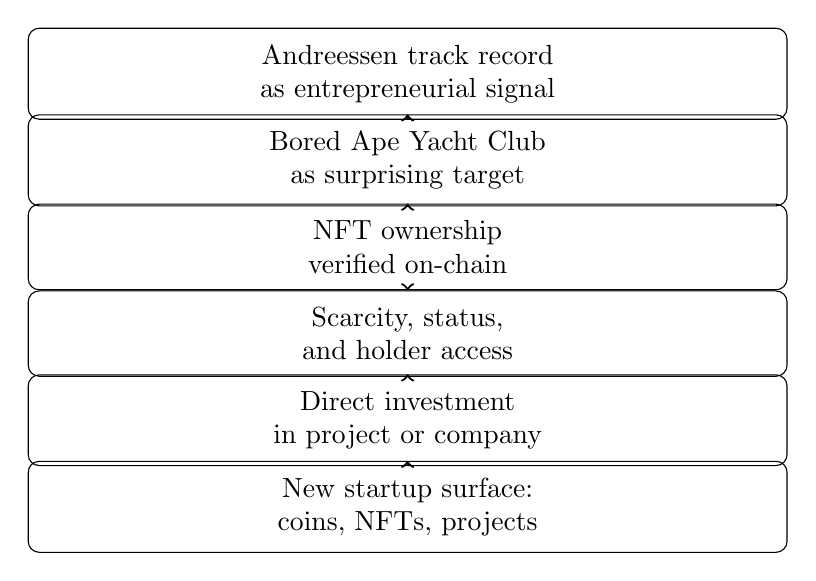
\begin{tikzpicture}[
  node distance=0.75cm,
  every node/.style={
    draw,
    rounded corners,
    align=center,
    text width=0.76\linewidth,
    inner sep=6pt
  },
  arrow/.style={->, thick}
]
\node (track) {Andreessen track record\\as entrepreneurial signal};
\node (bayc) [below of=track, yshift=-0.35cm] {Bored Ape Yacht Club\\as surprising target};
\node (verify) [below of=bayc, yshift=-0.35cm] {NFT ownership\\verified on-chain};
\node (access) [below of=verify, yshift=-0.35cm] {Scarcity, status,\\and holder access};
\node (company) [below of=access, yshift=-0.35cm] {Direct investment\\in project or company};
\node (startup) [below of=company, yshift=-0.35cm] {New startup surface:\\coins, NFTs, projects};

\draw[arrow] (track) -- (bayc);
\draw[arrow] (bayc) -- (verify);
\draw[arrow] (verify) -- (access);
\draw[arrow] (access) -- (company);
\draw[arrow] (company) -- (startup);
\end{tikzpicture}
\caption{A transcript-derived reconstruction of the lecture's mechanism: the investor's track record turns attention toward BAYC; NFT verification supports scarcity and access; the business question then shifts toward project-level investment.}
\end{figure}

\section{Asset Exposure Versus Company Exposure}

The next pivot is the most important entrepreneurial move in the lecture. Up to this point, buying an NFT means buying the asset and hoping that the asset appreciates or gives useful holder benefits. The narrator then asks what changes if one invests directly in the project or company behind the NFT ecosystem.

The transcript gives a claimed investment scale:
\begin{equation}
I_{\mathrm{Andreessen}} \sim \$4\mathrm{B} \text{ to } \$5\mathrm{B}.
\end{equation}
This number should remain marked as a lecture claim. Its function in the chapter is to signal magnitude, not to establish a verified transaction value.

\subsection{Question \& Answer}

\paragraph{Question.}
What changes when the investment target is the project or company rather than the NFT itself?

\paragraph{Answer.}
The exposure changes. Buying the NFT gives exposure to the asset: its resale price, its status, and its access benefits. Investing in the project or company gives exposure to the business system being built around the assets.

We can write the distinction as:
\begin{align}
E_{\mathrm{asset}}
&\approx
\Delta P_{\mathrm{NFT}} + B_{\mathrm{holder}}, \\
E_{\mathrm{company}}
&\approx
R_{\mathrm{ecosystem}}.
\end{align}
Here \(E_{\mathrm{asset}}\) is asset exposure, \(\Delta P_{\mathrm{NFT}}\) is appreciation or depreciation of the NFT, and \(B_{\mathrm{holder}}\) represents holder benefits. \(E_{\mathrm{company}}\) is project or company exposure, and \(R_{\mathrm{ecosystem}}\) denotes returns from the larger business built around the community, brand, software, events, marketplaces, or access structure.

This is the chapter's central analytical distinction. The lecture is not merely saying, ``NFTs are expensive.'' It is saying that a new investment surface may appear when the asset, the community, and the operating company become separable targets of capital.

\paragraph{Worked classification.}
Suppose an investor has three possible targets:
\begin{equation}
\mathcal{S}
=
\{\text{coins},\ \text{NFT assets},\ \text{NFT projects/companies}\}.
\end{equation}
The lecture's classification rule is:

\begin{enumerate}
\item If the investor buys Bitcoin or another cryptocurrency, the exposure is primarily to the coin's market value.
\item If the investor buys a Bored Ape NFT, the exposure is to the NFT's resale value and holder benefits.
\item If the investor invests in the project or company behind the NFT ecosystem, the exposure is to the enterprise being built around that ecosystem.
\end{enumerate}

So the same theme, crypto ownership, separates into three different commercial objects:
\begin{equation}
\text{coin} \neq \text{NFT asset} \neq \text{NFT project/company}.
\end{equation}
That is the clean version of the lecture's ``Pandora's box'' point.

\section{Startup Surface Area}

The lecture closes by widening the frame. If capital can move not only into coins and NFTs but also into NFT projects, then there is room for new financial interfaces. The narrator imagines a future in which one tab trades coins, another trades NFTs, and another lets investors choose between projects they want to fund.

We can describe the possible platform as an allocation map:
\begin{equation}
A:
\text{investor capital}
\longrightarrow
(\text{coins},\ \text{NFTs},\ \text{projects}).
\end{equation}
An investor who previously had two obvious crypto choices, coins or NFTs, is now imagined as having a third:
\begin{equation}
\text{old menu} = \{\text{coins},\ \text{NFTs}\},
\qquad
\text{new menu} = \{\text{coins},\ \text{NFTs},\ \text{projects}\}.
\end{equation}

The late transcript becomes noisy around examples such as hotel keys, private keys, playlists, and other utilities. We should not build a detailed theory from that garbled material. The stable idea is enough: NFT ownership may be a gateway to commercial systems, and those systems may themselves become investable.

\begin{figure}
\centering
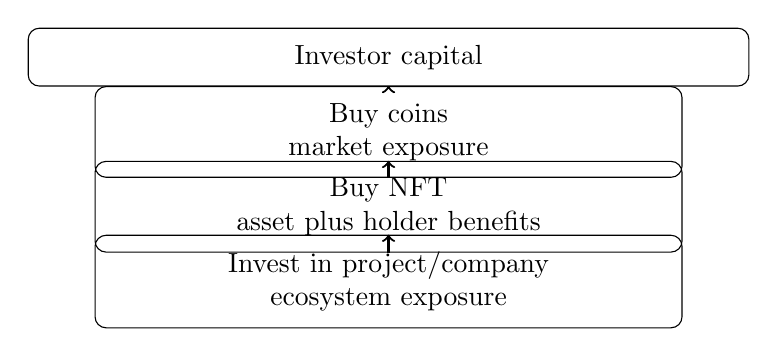
\begin{tikzpicture}[
  node distance=0.7cm,
  box/.style={
    draw,
    rounded corners,
    align=center,
    text width=0.72\linewidth,
    inner sep=6pt
  },
  smallbox/.style={
    draw,
    rounded corners,
    align=center,
    text width=0.58\linewidth,
    inner sep=6pt
  },
  arrow/.style={->, thick}
]
\node[box] (capital) {Investor capital};
\node[smallbox] (coins) [below of=capital, yshift=-0.25cm] {Buy coins\\market exposure};
\node[smallbox] (nft) [below of=coins, yshift=-0.25cm] {Buy NFT\\asset plus holder benefits};
\node[smallbox] (project) [below of=nft, yshift=-0.25cm] {Invest in project/company\\ecosystem exposure};

\draw[arrow] (capital) -- (coins);
\draw[arrow] (coins) -- (nft);
\draw[arrow] (nft) -- (project);
\end{tikzpicture}
\caption{A pocket-sized reconstruction of the investment menu described in the lecture. The main innovation is the third category: project or company exposure rather than only token or NFT ownership.}
\end{figure}

\section{Summary}

The lecture's movement is simple but important. First, it establishes Andreessen as a signal. Then it introduces Bored Ape Yacht Club as a surprising object of serious capital. The puzzle is resolved by reframing NFTs as verifiable ownership, and then by showing how scarcity, status, and access can attach to that ownership.

The deeper entrepreneurial point is the shift from buying the asset to investing in the structure behind the asset. In notation, the chapter's spine is:
\begin{equation}
\text{verified ownership}
\longrightarrow
\text{exclusive access}
\longrightarrow
\text{project-level business}
\longrightarrow
\text{new startup surface}.
\end{equation}
That is the durable claim to preserve. The monkey picture is the wrapper. The mechanism is the conversion of digital ownership into a business system that investors may want to fund directly.